\documentclass{article}

\usepackage[letterpaper,margin=1in]{geometry}
\usepackage[skip=12pt]{parskip}
\usepackage{sourcecodepro}

\usepackage{graphicx}
\usepackage{svg}
\usepackage{listings}
\usepackage{tikz}
\usetikzlibrary{shapes}

\usepackage{color}
\definecolor{orange}{rgb}{0.8,0.3,0.0}
\definecolor{blue}{rgb}{0.2,0.4,0.6}
\definecolor{gray}{rgb}{0.5,0.5,0.5}

\title{Lab 1 -- Prefix Scan and Barriers}
\author{Jerry Reinoehl}
\date{CS380P Fall 2023}

\begin{document}

\maketitle{}

\section{Prefix Scan Implementation}
To implement parallel prefix scan I used the Blelloch algorithm.
First we divide the elements among the threads according to
\[B = \Bigg\lceil\frac{N}{T}\Bigg\rceil = \Bigg\lfloor\frac{N+T-1}{T}\Bigg\rfloor\]
where $B$ is the block size, $N$ the number of elements, and $T$ the number of
threads.
To make the implementation a bit simpler and to avoid index-out-of-range
errors, we allocate $B * T$ elements for both \texttt{\small input\_vals} and
\texttt{\small output\_vals}.
This allows all threads to operate on the same number of elements, and if the
number of elements doesn't evenly divide the number of threads, extra zeroes are
added only to the final thread without altering the final result.

\begin{lstlisting}[
  language=c++,basicstyle=\small\ttfamily,breaklines=false,frame=tlbr,float=htbp,
  keywordstyle=\color{orange},commentstyle=\color{gray},
  emph={n_vals,n_threads,block_size},emphstyle=\color{blue}
]
int block_size = (*n_vals + args->n_threads - 1) / args->n_threads; // ceil(N/T)
int output_size = block_size * args->n_threads;

// Allocate input and output arrays
*input_vals = (int*) calloc(output_size, sizeof(int));
*output_vals = (int*) calloc(output_size, sizeof(int));
\end{lstlisting}

Here, we initialized the extra elements with zeroes for the prefix sum,
however, if we were to perform a different operation, such as multiplication,
it is important to note that we must initialize with the identity value for
our operation (e.g. 1's for multiplication).

The first step of the prefix scan is for each thread to perform a sequential
scan on its own block of elements.
This step also copies the input values to the output array so we may continue the
scan in place.
We allow all threads to synchronize as later steps are dependent on the
values that are calculated here.
This results in $O(N)$ operations in $O(N/T)$ time.

\begin{lstlisting}[
  language=c++,basicstyle=\small\ttfamily,breaklines=false,frame=tlbr,float=htbp,
  keywordstyle=\color{orange},commentstyle=\color{gray},
  emph={input,output,wait,op},emphstyle=\color{blue}
]
// Perform prefix scan on our block of data.
int x, y;
x = input[block_start];
output[block_start] = x;
for (int i = 1; i < block_size; i++) {
  y = input[block_start + i];
  x = op(x, y, n_loops);
  output[block_start + i] = x;
}

barrier->wait();
\end{lstlisting}

Next, we perform the up-sweep.
We select every second thread and have it combine its sum with the previous
thread's sum, and synchronize.
We then select every fourth thread and combine it with the thread with an ID of
two less than the current thread.
We continue this operation, doubling the stride until the stride is greater
than the number of threads.
The up-sweep performs $O(T)$ operations in $O(\log{T})$ time.

\begin{center}
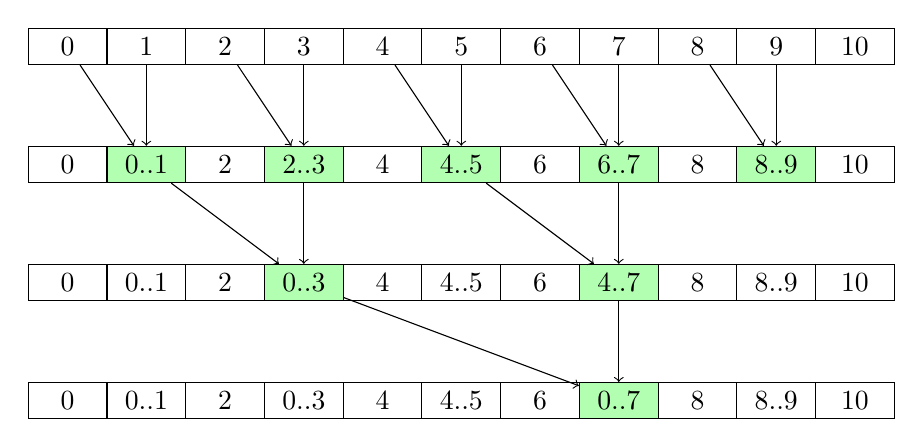
\begin{tikzpicture}
  \node[draw,rectangle,minimum width=10mm,minimum height=3mm] at (0,0) (n0-0) {0};
  \node[draw,rectangle,minimum width=10mm,minimum height=3mm] at (1,0) (n0-1) {1};
  \node[draw,rectangle,minimum width=10mm,minimum height=3mm] at (2,0) (n0-2) {2};
  \node[draw,rectangle,minimum width=10mm,minimum height=3mm] at (3,0) (n0-3) {3};
  \node[draw,rectangle,minimum width=10mm,minimum height=3mm] at (4,0) (n0-4) {4};
  \node[draw,rectangle,minimum width=10mm,minimum height=3mm] at (5,0) (n0-5) {5};
  \node[draw,rectangle,minimum width=10mm,minimum height=3mm] at (6,0) (n0-6) {6};
  \node[draw,rectangle,minimum width=10mm,minimum height=3mm] at (7,0) (n0-7) {7};
  \node[draw,rectangle,minimum width=10mm,minimum height=3mm] at (8,0) (n0-8) {8};
  \node[draw,rectangle,minimum width=10mm,minimum height=3mm] at (9,0) (n0-9) {9};
  \node[draw,rectangle,minimum width=10mm,minimum height=3mm] at (10,0) (n0-10) {10};

  \node[draw,rectangle,minimum width=10mm,minimum height=3mm] at (0,-1.5) (n1-0) {0};
  \node[draw,rectangle,minimum width=10mm,minimum height=3mm,fill=green!30] at (1,-1.5) (n1-1) {0..1};
  \node[draw,rectangle,minimum width=10mm,minimum height=3mm] at (2,-1.5) (n1-2) {2};
  \node[draw,rectangle,minimum width=10mm,minimum height=3mm,fill=green!30] at (3,-1.5) (n1-3) {2..3};
  \node[draw,rectangle,minimum width=10mm,minimum height=3mm] at (4,-1.5) (n1-4) {4};
  \node[draw,rectangle,minimum width=10mm,minimum height=3mm,fill=green!30] at (5,-1.5) (n1-5) {4..5};
  \node[draw,rectangle,minimum width=10mm,minimum height=3mm] at (6,-1.5) (n1-6) {6};
  \node[draw,rectangle,minimum width=10mm,minimum height=3mm,fill=green!30] at (7,-1.5) (n1-7) {6..7};
  \node[draw,rectangle,minimum width=10mm,minimum height=3mm] at (8,-1.5) (n1-8) {8};
  \node[draw,rectangle,minimum width=10mm,minimum height=3mm,fill=green!30] at (9,-1.5) (n1-9) {8..9};
  \node[draw,rectangle,minimum width=10mm,minimum height=3mm] at (10,-1.5) (n1-10) {10};

  \draw[->] (n0-0) -- (n1-1); \draw[->] (n0-1) -- (n1-1);
  \draw[->] (n0-2) -- (n1-3); \draw[->] (n0-3) -- (n1-3);
  \draw[->] (n0-4) -- (n1-5); \draw[->] (n0-5) -- (n1-5);
  \draw[->] (n0-6) -- (n1-7); \draw[->] (n0-7) -- (n1-7);
  \draw[->] (n0-8) -- (n1-9); \draw[->] (n0-9) -- (n1-9);

  \node[draw,rectangle,minimum width=10mm,minimum height=3mm] at (0,-3) (n2-0) {0};
  \node[draw,rectangle,minimum width=10mm,minimum height=3mm] at (1,-3) (n2-1) {0..1};
  \node[draw,rectangle,minimum width=10mm,minimum height=3mm] at (2,-3) (n2-2) {2};
  \node[draw,rectangle,minimum width=10mm,minimum height=3mm,fill=green!30] at (3,-3) (n2-3) {0..3};
  \node[draw,rectangle,minimum width=10mm,minimum height=3mm] at (4,-3) (n2-4) {4};
  \node[draw,rectangle,minimum width=10mm,minimum height=3mm] at (5,-3) (n2-5) {4..5};
  \node[draw,rectangle,minimum width=10mm,minimum height=3mm] at (6,-3) (n2-6) {6};
  \node[draw,rectangle,minimum width=10mm,minimum height=3mm,fill=green!30] at (7,-3) (n2-7) {4..7};
  \node[draw,rectangle,minimum width=10mm,minimum height=3mm] at (8,-3) (n2-8) {8};
  \node[draw,rectangle,minimum width=10mm,minimum height=3mm] at (9,-3) (n2-9) {8..9};
  \node[draw,rectangle,minimum width=10mm,minimum height=3mm] at (10,-3) (n2-10) {10};

  \draw[->] (n1-1) -- (n2-3); \draw[->] (n1-3) -- (n2-3);
  \draw[->] (n1-5) -- (n2-7); \draw[->] (n1-7) -- (n2-7);

  \node[draw,rectangle,minimum width=10mm,minimum height=3mm] at (0,-4.5) (n3-0) {0};
  \node[draw,rectangle,minimum width=10mm,minimum height=3mm] at (1,-4.5) (n3-1) {0..1};
  \node[draw,rectangle,minimum width=10mm,minimum height=3mm] at (2,-4.5) (n3-2) {2};
  \node[draw,rectangle,minimum width=10mm,minimum height=3mm] at (3,-4.5) (n3-3) {0..3};
  \node[draw,rectangle,minimum width=10mm,minimum height=3mm] at (4,-4.5) (n3-4) {4};
  \node[draw,rectangle,minimum width=10mm,minimum height=3mm] at (5,-4.5) (n3-5) {4..5};
  \node[draw,rectangle,minimum width=10mm,minimum height=3mm] at (6,-4.5) (n3-6) {6};
  \node[draw,rectangle,minimum width=10mm,minimum height=3mm,fill=green!30] at (7,-4.5) (n3-7) {0..7};
  \node[draw,rectangle,minimum width=10mm,minimum height=3mm] at (8,-4.5) (n3-8) {8};
  \node[draw,rectangle,minimum width=10mm,minimum height=3mm] at (9,-4.5) (n3-9) {8..9};
  \node[draw,rectangle,minimum width=10mm,minimum height=3mm] at (10,-4.5) (n3-10) {10};

  \draw[->] (n2-3) -- (n3-7); \draw[->] (n2-7) -- (n3-7);

\end{tikzpicture}
\end{center}

\begin{lstlisting}[
  language=c++,basicstyle=\small\ttfamily,breaklines=false,frame=tlbr,float=htbp,
  keywordstyle=\color{orange},commentstyle=\color{gray},
  emph={input,output,wait,op,stride},emphstyle=\color{blue}
]
// Compute up-sweep.
for (stride = 1; stride < n_threads; stride <<= 1) {
  if ((t_id + 1) % (stride << 1) == 0) {
    x = output[block_end - stride * block_size];
    y = output[block_end];
    output[block_end] = op(x, y, n_loops);
  }
  barrier->wait();
}
\end{lstlisting}

We then compute the down-sweep.
We select every \texttt{\small stride * 2} threads and have it combine its sum
with the thread \texttt{\small stride} units greater, and divide the stride by 2.
We continue while the stride is greater than 0.
Similar to the up-sweep, the down-sweep does $O(T)$ operations in $O(\log{T})$
time.

\begin{center}
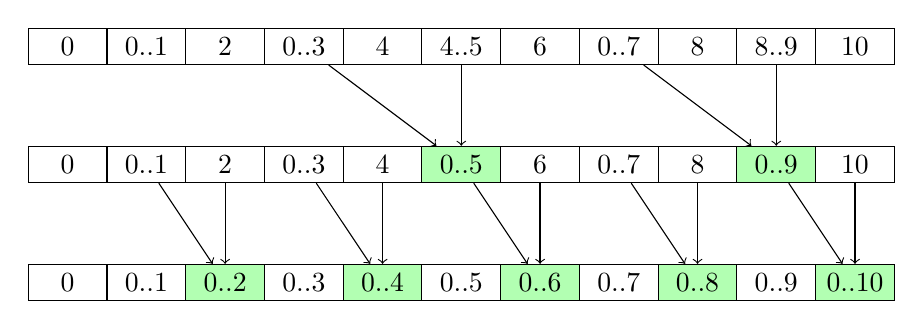
\begin{tikzpicture}

  \node[draw,rectangle,minimum width=10mm,minimum height=3mm] at (0,0) (n4-0) {0};
  \node[draw,rectangle,minimum width=10mm,minimum height=3mm] at (1,0) (n4-1) {0..1};
  \node[draw,rectangle,minimum width=10mm,minimum height=3mm] at (2,0) (n4-2) {2};
  \node[draw,rectangle,minimum width=10mm,minimum height=3mm] at (3,0) (n4-3) {0..3};
  \node[draw,rectangle,minimum width=10mm,minimum height=3mm] at (4,0) (n4-4) {4};
  \node[draw,rectangle,minimum width=10mm,minimum height=3mm] at (5,0) (n4-5) {4..5};
  \node[draw,rectangle,minimum width=10mm,minimum height=3mm] at (6,0) (n4-6) {6};
  \node[draw,rectangle,minimum width=10mm,minimum height=3mm] at (7,0) (n4-7) {0..7};
  \node[draw,rectangle,minimum width=10mm,minimum height=3mm] at (8,0) (n4-8) {8};
  \node[draw,rectangle,minimum width=10mm,minimum height=3mm] at (9,0) (n4-9) {8..9};
  \node[draw,rectangle,minimum width=10mm,minimum height=3mm] at (10,0) (n4-10) {10};

  \node[draw,rectangle,minimum width=10mm,minimum height=3mm] at (0,-1.5) (n5-0) {0};
  \node[draw,rectangle,minimum width=10mm,minimum height=3mm] at (1,-1.5) (n5-1) {0..1};
  \node[draw,rectangle,minimum width=10mm,minimum height=3mm] at (2,-1.5) (n5-2) {2};
  \node[draw,rectangle,minimum width=10mm,minimum height=3mm] at (3,-1.5) (n5-3) {0..3};
  \node[draw,rectangle,minimum width=10mm,minimum height=3mm] at (4,-1.5) (n5-4) {4};
  \node[draw,rectangle,minimum width=10mm,minimum height=3mm,fill=green!30] at (5,-1.5) (n5-5) {0..5};
  \node[draw,rectangle,minimum width=10mm,minimum height=3mm] at (6,-1.5) (n5-6) {6};
  \node[draw,rectangle,minimum width=10mm,minimum height=3mm] at (7,-1.5) (n5-7) {0..7};
  \node[draw,rectangle,minimum width=10mm,minimum height=3mm] at (8,-1.5) (n5-8) {8};
  \node[draw,rectangle,minimum width=10mm,minimum height=3mm,fill=green!30] at (9,-1.5) (n5-9) {0..9};
  \node[draw,rectangle,minimum width=10mm,minimum height=3mm] at (10,-1.5) (n5-10) {10};

  \draw[->] (n4-3) -- (n5-5); \draw[->] (n4-5) -- (n5-5);
  \draw[->] (n4-7) -- (n5-9); \draw[->] (n4-9) -- (n5-9);

  \node[draw,rectangle,minimum width=10mm,minimum height=3mm] at (0,-3) (n6-0) {0};
  \node[draw,rectangle,minimum width=10mm,minimum height=3mm] at (1,-3) (n6-1) {0..1};
  \node[draw,rectangle,minimum width=10mm,minimum height=3mm,fill=green!30] at (2,-3) (n6-2) {0..2};
  \node[draw,rectangle,minimum width=10mm,minimum height=3mm] at (3,-3) (n6-3) {0..3};
  \node[draw,rectangle,minimum width=10mm,minimum height=3mm,fill=green!30] at (4,-3) (n6-4) {0..4};
  \node[draw,rectangle,minimum width=10mm,minimum height=3mm] at (5,-3) (n6-5) {0..5};
  \node[draw,rectangle,minimum width=10mm,minimum height=3mm,fill=green!30] at (6,-3) (n6-6) {0..6};
  \node[draw,rectangle,minimum width=10mm,minimum height=3mm] at (7,-3) (n6-7) {0..7};
  \node[draw,rectangle,minimum width=10mm,minimum height=3mm,fill=green!30] at (8,-3) (n6-8) {0..8};
  \node[draw,rectangle,minimum width=10mm,minimum height=3mm] at (9,-3) (n6-9) {0..9};
  \node[draw,rectangle,minimum width=10mm,minimum height=3mm,fill=green!30] at (10,-3) (n6-10) {0..10};

  \draw[->] (n5-1) -- (n6-2); \draw[->] (n5-2) -- (n6-2);
  \draw[->] (n5-3) -- (n6-4); \draw[->] (n5-4) -- (n6-4);
  \draw[->] (n5-5) -- (n6-6); \draw[->] (n5-6) -- (n6-6);
  \draw[->] (n5-7) -- (n6-8); \draw[->] (n5-8) -- (n6-8);
  \draw[->] (n5-9) -- (n6-10); \draw[->] (n5-10) -- (n6-10);

\end{tikzpicture}
\end{center}

\begin{lstlisting}[
  language=c++,basicstyle=\small\ttfamily,breaklines=false,frame=tlbr,float=htbp,
  keywordstyle=\color{orange},commentstyle=\color{gray},
  emph={input,output,wait,op,stride},emphstyle=\color{blue}
]
// Compute down-sweep.
for (stride = stride >> 1; stride > 0; stride >>= 1) {
  if ((t_id + 1) % (stride << 1) == 0 && (t_id + stride) < n_threads) {
    x = output[block_end + stride * block_size];
    y = output[block_end];
    output[block_end + stride * block_size] = op(x, y, n_loops);
  }
  barrier->wait();
}
\end{lstlisting}

Finally, each thread computes the final results for its block by adding the
computed sum of the previous thread to each of its block's elements except for
the last, which already contains the correct sum.
This final step performs $O(N)$ operations in $O(N/T)$ time.

\begin{lstlisting}[
  language=c++,basicstyle=\small\ttfamily,breaklines=false,frame=tlbr,float=htbp,
  keywordstyle=\color{orange},commentstyle=\color{gray},
  emph={input,output,wait,op,stride},emphstyle=\color{blue}
]
// Finalize prefix sum for our block. Add the sum from the previous block
// to all of our elements except for the last.
if (t_id > 0) {
  for (int i = 1; i < block_size; i++) {
    x = output[block_end - i];
    y = output[block_end - block_size];
    output[block_end - i] = op(x, y, n_loops);
  }
}
\end{lstlisting}

The total number of operations comes to $O(2N + 2T)$ in time
$O(\frac{2N}{T} + 2\log{T})$, or $O(N)$ and $O(N/T)$ for large $N$.
The algorithm is work efficient because it does not do more operations
asymptotically than the sequential implementation.

\section{Parallel Prefix Scan Results}

The following graphs depict the execution time of the parallel prefix scan,
with 100,000 loops, for 1k, 8k, and 16k elements.
The dashed line indicates the running time of the sequential prefix scan.
These tests were run on a 16 core CPU, and you can see we have a steady
improvement in performance until we run with more threads than the CPU actually
has.
At this point, running with more threads only adds more overhead as we can
still only run 16 threads simultaneously, but must now incur the cost of
creating and destroying more threads as well as the cost of contention at the
barrier.
This indicates that for best performance we should set the number of threads to
the number of CPU core we actually have.

\begin{figure}[float=htbp]
  \includesvg[scale=0.5]{pthread-time-1k.svg}
  \includesvg[scale=0.5]{pthread-time-8k.svg}
\end{figure}
\begin{center}
  \includesvg[scale=0.5]{pthread-time-16k.svg}
\end{center}

The graph below shows the speedup results, again for 100,000 loops.
The dashed line indicates the ideal speedup.
Again, we notice a peak at 16 threads, and also while we can attain a good
speedup, we are not achieving the ideal speedup due to overhead and contention.
We also note that we can get better speedup by increasing the number of
elements.

%\begin{center}
%  \includesvg[scale=1.0]{pthread-speedup.svg}
%\end{center}
\begin{center}
  \includegraphics[scale=0.2]{pthread-speedup.png}
\end{center}

By varying the number of loops we can find where the parallel implementation is
no longer faster than the sequential scan.
We see that at roughly 65 loops the parallel and sequential implementations run
in about the same time.
This suggests that the amount of work performed by the operator affects the
speedup attained by incorporating parallelism.
Parallelism is more effective when we want to parallelize longer running, more
compute intensive operations, rather than simple ones, such as scalar addition.
We want to amortize the overhead costs with a longer running computation to
achieve a performance gain.

\begin{center}
  \includesvg[scale=0.8]{pthread-time-16k-l10.svg}
\end{center}

\section{Barrier Implementation}

My barrier implementation is based on a mutex and an array of go integers.
Upon entering the barrier, a thread would grab the lock, decrement the count,
grab its go bit, and check if the count became zero.
If the count is now zero, it will reset the count, and flip all go bits, thus
signaling to all awaiting threads that they may proceed.
If the count is not yet zero, the thread would spin waiting for its go bit to
flip.

I did find that simply spinning was good for performance up to the number of
threads of the machine, however, when setting the number of threads greater,
spinning often resulted in execution time much slower than the equivalent
\texttt{\small pthread\_barrier} scan.
This was due to threads hogging the core and not yielding the CPU to the
threads it was waiting on.

To fix this problem I added a \texttt{\small sleep(0)} to yield the CPU.
While this greatly improved performance for threads greater than 16, it did
hurt performance for threads 16 or less due to additional context switches.
I was able to find a middle ground by spinning only the number of threads of
the machine, and yielding the first threads that showed up.
For example, if running with 20 threads, the first 4 threads would yield, while
the remaining 16 threads would spin.
This achieved similar performance for threads less than 16 because no threads
would yield, and also achieved much better performance when setting the number
of threads to something greater.

\begin{lstlisting}[
  language=c++,basicstyle=\small\ttfamily,breaklines=false,frame=tlbr,float=htbp,
  keywordstyle=\color{orange},commentstyle=\color{gray},
  emph={wait,go,count},emphstyle=\color{blue}
]
static const int HARDWARE_CONCURRENCY = std::thread::hardware_concurrency();

inline void SpinBarrier::wait() {
  int count;
  int go;

  pthread_mutex_lock(&count_lock_);
  count = --count_;
  go = !go_[count];

  if (count == 0) {
    pthread_mutex_unlock(&count_lock_);
    count_ = go_len_;
    for (int i = go_len_ - 1; i >= 0; i--)
      go_[i] = go; // flip go ints
  } else {
    pthread_mutex_unlock(&count_lock_);
    while(go_[count] != go) {
      if (count >= HARDWARE_CONCURRENCY) {
        sleep(0);  // yield cpu
      }
    }
  }
}
\end{lstlisting}

\begin{center}
  \includesvg[scale=0.8]{spin-time-impl.svg}
\end{center}

The \texttt{\small pthread\_barrier\_t} implementation is very similar to my
own, with the difference being that, instead of an array of go bits to wait
upon, it uses a condition variable.
When a thread waits for the condition variable, it will be put to sleep until
signaled by the corresponding broadcast.
Whereas, with my implementation, we may yield the thread only to be rescheduled
later and again re-yield.
This hurts performance due to additional context switching.
This is why we see faster execution times from the pthread barrier
implementation above when the number of threads is greater than 16.
However, because my implementation does not yield when the number of threads is
less than the number of machine threads it has slightly better performance for
threads less than or equal to 16.

The takeaway here is that if we are executing many threads, maybe over many
programs, it is better to yield to give the CPU to the threads you are waiting
on.
However, for better performance we can just spin with a number of threads equal
to the number of CPU cores.

\begin{center}
  \includesvg[scale=1.0]{spin-speedup.svg}
\end{center}

\begin{center}
  \includesvg[scale=0.8]{spin-time-16k-l10.svg}
\end{center}

\begin{center}
  \begin{tabular}{|l|c|}
    \hline
    \multicolumn{2}{|c|}{\bf Time Breakdown} \\ \hline
    Prefix Scan Impl & 15 hrs \\ \hline
    Barrier Impl & 8 hrs      \\ \hline
    Report & 10 hrs           \\ \hline
    \bf{Total} & \bf{32 hrs}  \\ \hline
  \end{tabular}
\end{center}

\end{document}
